\chapter{Perubahan Global dan Biosfer}\label{ch:b2:global-change}

Antara tahun 1851 dan 1858 Henry Thoreau berjalan menyusuri hutan dan
padang di sekitar Concord, Massachusetts, lalu menuliskan hari tiap
tumbuhan dari sekitar lima ratus tumbuhan pertama kali berbunga. Satu
setengah abad kemudian, para ahli botani kembali ke tempat yang sama
dengan buku catatannya. Beri biru semak tinggi yang dilihat Thoreau
membuka pada 11 Mei kini membuka pada 12 April; seluruh floranya
berbunga, secara rerata, sepuluh hari lebih awal daripada pada zamannya,
seiring dengan sebuah musim semi yang \qty{2.4}{\celsius} lebih hangat;
dan seperempat spesiesnya telah lenyap dari Concord --- bukan secara
acak, melainkan spesies yang pembungaannya tidak dapat mengikuti
suhunya. Bab sebelumnya memberikan mesinnya: daur pada
\cref{ch:b2:biogeochemical-cycles}, seleksi dan hanyutan pada
\cref{ch:b2:population-genetics}, persaingan dan spesiasi pada
\cref{ch:b2:speciation}, \omterm{def:b2:living-soil:soil}{tanah} pada \cref{ch:b2:living-soil}. Bab ini
menaruh sebuah angka pada apa yang sedang terjadi kepada makhluk hidup
ketika satu spesies mengubah kimia udara dan lautnya: berapa banyak
pemanasan tiap ton karbon, berapa hari musim semi tiap derajat, berapa
meter ke atas bukit, berapa banyak asam di lautnya, berapa banyak
spesies tiap hektar yang hilang --- dan apa yang dikatakan angkanya
tentang abad di depannya.

\section{Perubahan fisiknya}

\begin{proposition}[Pemanasannya sebanding dengan pancaran kumulatifnya]\label{prop:b2:global-change:tcre}
\index{pemanasan global}\index{pancaran kumulatif}%
\index{anggaran karbon}\index{efek rumah kaca}
Karbon dioksida menyerap inframerah yang dipancarkan \omterm{def:b2:living-soil:soil}{tanahnya} lalu
mengembalikan sebagiannya; lebih banyak \ensuremath{\mathrm{CO_2}} berarti sebuah
permukaan yang lebih hangat, sebesar kira-kira \qty{3}{\celsius} tiap
pelipatduaan setelah lautannya menyusul (yaitu \emph{kepekaan
iklimnya}). Karena tanggapan suhunya terhadap \ensuremath{\mathrm{CO_2}} bersifat
logaritmik terhadap kepekatannya sementara bagian pancaran yang
mengudara turun ketika kepekatannya naik, kedua kelengkungannya nyaris
saling meniadakan, dan pemanasan rerata globalnya, sampai sebuah
hampiran yang baik, bersifat \emph{lurus terhadap jumlah kumulatif
karbon yang dipancarkan}, apa pun waktunya:
\[
\Delta T \approx \lambda\,C_{\text{kum}}, \qquad \lambda \approx
\qty{1.65}{\celsius} \text{ tiap } \qty{1000}{GtC}
\]
(\qty{0.45}{\celsius} tiap \qty{1000}{Gt} \ensuremath{\mathrm{CO_2}}). Sekitar
\qty{700}{GtC} yang dipancarkan sejak tahun 1850 telah menghangatkan
planetnya sebesar \qty{1.2}{\celsius} --- dan hubungannya memberikan
tiap sasarannya sebuah anggaran: \qty{1.5}{\celsius} membolehkan
kira-kira \qty{900}{GtC} seluruhnya, yaitu \qty{200}{GtC} lebih banyak
daripada yang telah dipancarkan, yakni dua puluh tahun pada laju
sekarang. Pemanasannya tidak merata: dua kali reratanya di daratan dan
tiga kali di Arktiknya; malamnya lebih daripada siangnya; dan ia datang
bersama sisanya --- hujan yang lebih deras dan kekeringan yang lebih
panjang, muka laut yang naik \qty{4}{mm} tiap tahun, es yang seperlima
lebih kecil pada musim panas, dan sebuah lautan yang telah menyerap
\qty{90}{\%} panasnya dan seperempat karbonnya.
\end{proposition}
\begin{proof}[Bukti eksperimental]
Kesebandingannya ditemukan pada model iklim dengan kerumitan apa pun
lalu dibenarkan catatan yang teramati: menggambarkan pemanasannya sejak
tahun 1850 terhadap \omterm{prop:b2:global-change:tcre}{pancaran kumulatifnya} memberikan sebuah garis lurus
lewat dasawarsanya. \omterm{prop:b2:global-change:tcre}{Efek rumah kacanya} sendiri terukur dari orbit:
satelit melihat inframerah yang dipancarkan Bumi dengan pita serapan
\ensuremath{\mathrm{CO_2}}, metana, dan uap airnya terpotong darinya, dan potongannya
telah mendalam antara tahun 1970 dan 2020 tepat sebesar yang diramalkan
kenaikan gas ini. Isotop dan oksigen yang turun pada
\cref{ch:b2:biogeochemical-cycles} mengikatkan \ensuremath{\mathrm{CO_2}} tambahannya
kepada bahan bakar fosilnya.
\end{proof}

\begin{omfigure}
\begin{tikzpicture}
\begin{axis}[
  width=0.88\linewidth, height=5.6cm,
  axis x line=bottom, axis y line=left,
  xmin=1845, xmax=2030, ymin=-0.3, ymax=1.5,
  xlabel={dasawarsa}, ylabel={pemanasan (\unit{\celsius}) sejak 1850--1900},
  xlabel style={font=\small, at={(axis description cs:0.5,-0.13)}, anchor=north},
  ylabel style={font=\small},
  tick label style={font=\small}, xtick={1850,1900,1950,2000}, ytick={0,0.5,1,1.5},
  scaled x ticks=false, x tick label style={/pgf/number format/1000 sep=},
  clip=false,
]
\addplot[ybar, bar width=7pt, fill=omThm!50, draw=omThm] coordinates {
(1855,0.00) (1865,-0.04) (1875,0.02) (1885,-0.06) (1895,-0.02) (1905,-0.10) (1915,-0.06) (1925,0.05) (1935,0.15) (1945,0.25) (1955,0.15) (1965,0.15) (1975,0.18) (1985,0.40) (1995,0.55) (2005,0.78) (2015,1.02) (2023,1.28)};
\node[font=\scriptsize, anchor=west, align=left] at (axis cs:1850,1.2) {tiap batang: rerata sebuah dasawarsa; yang terakhir, 2020--2024\\ \qty{700}{GtC} dipancarkan, $\qty{1.65}{\celsius}/\qty{1000}{GtC}$: \qty{1.2}{\celsius}};
\end{axis}
\end{tikzpicture}

{\small Suhu permukaan rerata global menurut dasawarsa, terhadap
separuh kedua abad kesembilan belas. Empat dasawarsa terakhirnya
masing-masing mencetak rekor, dan kenaikannya sejak tahun 1970 adalah
\qty{0.2}{\celsius} tiap dasawarsa.}
\end{omfigure}

\section{Kalendernya: fenologi}

\begin{theorem}[Derajat-hari dan majunya musim semi]\label{thm:b2:global-change:phenology}
\index{fenologi}\index{derajat-hari}\index{waktu termal}\index{ketakserasian fenologi}
Banyak peristiwa dalam hidup tumbuhan dan hewan berdarah dingin ---
pecahnya tunas, pembungaan, penetasan telur, kemunculan --- terjadi
ketika \emph{\omterm{thm:b2:global-change:phenology}{waktu termal}} yang tertimbun sejak sebuah tanggal awal,
yaitu jumlah suhu harian di atas sebuah dasar $T_b$ (yaitu
\emph{derajat-hari}), mencapai sebuah jumlah tetap $K$. Jika suhu musim
seminya naik secara lurus, $T(t) = T_b
+ b\,(t - t_0)$ pada $b$ derajat
tiap hari sejak hari $t_0$ ia melewati dasarnya, peristiwanya terjadi
pada
\[
t^{*} = t_0 + \sqrt{2K/b},
\]
dan sebuah pemanasan seragam sebesar $\Delta T$ memajukan hari
pelintasannya sebesar $\Delta T/b$ beserta peristiwanya: dengan $b \approx
\qty{0.1}{\celsius}$ tiap hari, \emph{kira-kira sepuluh hari
lebih awal tiap derajat}. Spesies berbeda dalam $T_b$, $K$, dan dalam
apakah ia juga memakai panjang harinya, yang tidak diubah pemanasannya
--- sehingga anggota sebuah rantai makanan maju pada laju yang berbeda
dan waktunya terpisah: sebuah \emph{\omterm{thm:b2:global-change:phenology}{ketakserasian fenologi}} antara ulat
dan burung yang harus memberi makan anaknya dengan ulat itu.
\end{theorem}
\begin{proof}
Derajat-hari sejak $t_0$: $\int_{t_0}^{t}(T - T_b)\,\mathrm{d}t' =
b\,(t - t_0)^{2}/2$, yang sama dengan $K$ ketika $t - t_0 = \sqrt{2K/b}$. Pemanasan sebesar $\Delta T$ menggantikan $T$ dengan $T + \Delta T$: dasarnya dilewati $\Delta T/b$ hari lebih awal dan
penimbunannya, yang serupa sejak hari itu, rampung $\Delta T/b$ hari
lebih awal. (Jika pemanasannya juga mencuramkan $b$, selang
$\sqrt{2K/b}$-nya memendek juga.) Sebuah spesies yang berisyarat
panjang hari menjaga tanggalnya; yang berisyarat derajat-hari
berpindah; celah di antara keduanya bertambah sebesar $\Delta T/b$.
\end{proof}
\begin{proof}[Bukti eksperimental]
Flora Concord milik Thoreau, dan catatan keluarga Marsham berisi dua
puluh tujuh tanda musim semi di Norfolk yang disimpan dari tahun 1736
sampai 1947, keduanya memperlihatkan pembungaan dan pendaunan yang maju
sebesar \qtyrange{3}{6}{d} tiap derajat pemanasan musim seminya. \omterm{def:b2:angiosperm-reproduction:flower}{Bunga}
sakura Kyoto, yang ditanggali di buku harian istana sejak abad
kesembilan, bertahan di sekitar pertengahan April selama seribu tahun
lalu berpindah ke awal April sejak tahun 1900, dengan tanggal terawal
dalam catatannya jatuh pada tahun 2020-an. Di Belanda ulat pohon eknya
kini memuncak dua pekan lebih awal daripada pada tahun 1985; burung
gelatik besarnya, yang berisyarat kehangatan yang sama, telah
mengimbanginya, tetapi burung sikatan belangnya, yang mengatur waktu
ruayanya dari Afrika menurut panjang hari, tiba seperti sebelumnya lalu
mendapati puncaknya telah lewat --- populasinya telah turun sebesar
\qty{90}{\%} di tempat ketakserasiannya terbesar (Both dan rekannya,
2006).
\end{proof}

\begin{omfigure}
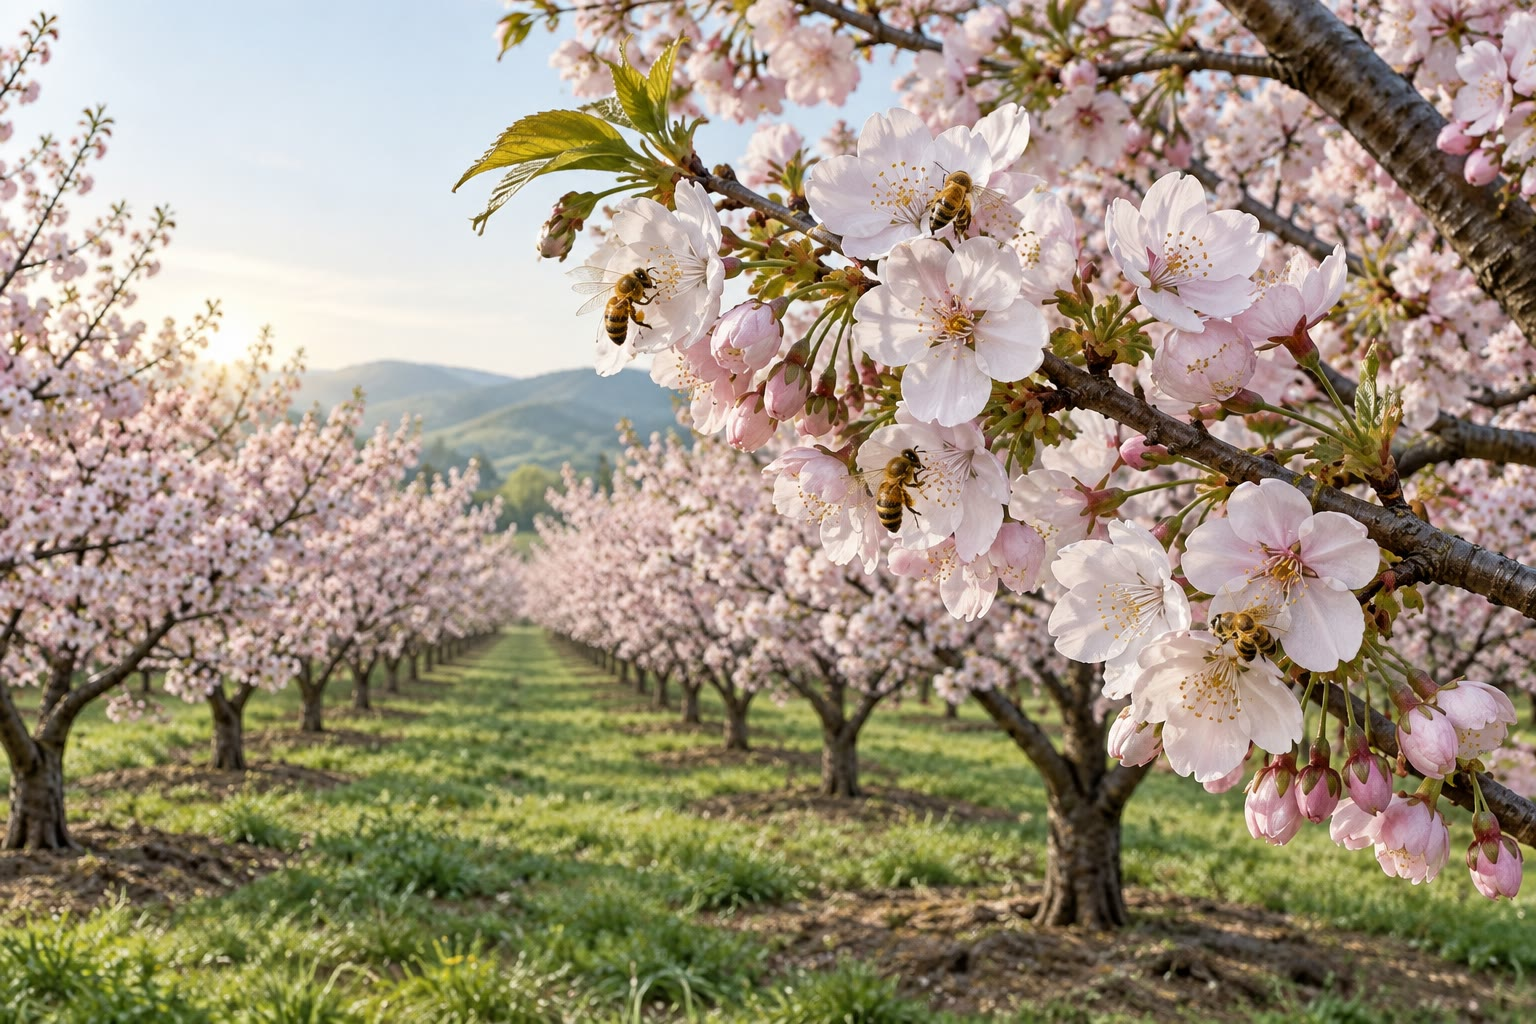
\includegraphics[width=0.62\linewidth]{images/book4/ai/b4-27-phenology-cherry.jpg}

{\small Sebuah kebun sakura yang sedang mekar. Sakura Kyoto, yang
ditanggali di buku harian selama dua belas abad, kini membuka lebih
awal daripada tahun mana pun sebelum 1900 --- dan lebah yang
menyerbukinya harus terbang pada hari yang sama.}
\end{omfigure}

\begin{omfigure}
\begin{tikzpicture}
\begin{axis}[
  width=0.74\linewidth, height=5.4cm,
  axis x line=bottom, axis y line=left,
  xmin=0, xmax=100, ymin=0, ymax=14,
  xlabel={hari sejak 1 Maret}, ylabel={suhu rerata harian (\unit{\celsius})},
  xlabel style={font=\small, at={(axis description cs:0.5,-0.13)}, anchor=north},
  ylabel style={font=\small},
  tick label style={font=\small}, xtick={0,20,40,60,80,100},
  legend style={font=\scriptsize, at={(0.03,0.97)}, anchor=north west, draw=none},
  clip=false,
]
\addplot[very thick, omDef, domain=0:100, samples=2] {2 + 0.1*x};
\addlegendentry{musim semi sebelum pemanasannya}
\addplot[very thick, omThm, domain=0:100, samples=2] {3 + 0.1*x};
\addlegendentry{musim semi yang \qty{1}{\celsius} lebih hangat}
\draw[dashed, gray] (axis cs:0,5) -- (axis cs:100,5); \node[font=\scriptsize, anchor=south east] at (axis cs:100,5) {suhu dasar $T_b = \qty{5}{\celsius}$};
\fill[omDef, opacity=0.15] (axis cs:30,5) -- (axis cs:93,5) -- (axis cs:93,11.3) -- cycle;
\fill[omThm, opacity=0.15] (axis cs:20,5) -- (axis cs:83,5) -- (axis cs:83,11.3) -- cycle;
\draw[<->, thick] (axis cs:83,1.6) -- (axis cs:93,1.6); \node[font=\scriptsize, anchor=south] at (axis cs:88,1.8) {10 hari};
\draw[dotted] (axis cs:93,0) -- (axis cs:93,5); \draw[dotted] (axis cs:83,0) -- (axis cs:83,5);
\node[font=\scriptsize, anchor=south, align=center] at (axis cs:62,11.4) {$K = 200$ derajat-hari\\ (luas yang terarsir)};
\end{axis}
\end{tikzpicture}

{\small Derajat-hari. Peristiwanya terjadi ketika luas yang terarsir
antara garis suhunya dan dasarnya mencapai $K$; sebuah musim semi yang
satu derajat lebih hangat melewati dasarnya sepuluh hari lebih cepat
lalu merampungkan jumlahnya sepuluh hari lebih cepat.}
\end{omfigure}

\section{Petanya: pergeseran sebaran}

\begin{proposition}[Isoterm berpindah, dan spesies mengikutinya]\label{prop:b2:global-change:range}
\index{pergeseran sebaran}\index{kecepatan iklim}\index{laju susut suhu}
Suhu turun kira-kira \qty{6.5}{\celsius} tiap kilometer ketinggian dan
kira-kira \qty{0.65}{\celsius} tiap seratus kilometer lintang di zona
sedangnya; karena itu sebuah pemanasan sebesar \qty{1}{\celsius}
memindahkan tiap isotermnya kira-kira \qty{150}{m} ke atas bukit dan
\qty{150}{km} ke arah kutubnya. Spesies yang batasnya ditetapkan
suhunya berpindah bersama isotermnya jika ia dapat: rerata ratusan
spesies yang dipelajari telah bergeser \qty{11}{m} ke atas bukit dan
\qty{17}{km} ke arah kutub tiap dasawarsa sejak tahun 1970, pada
kecepatan isotermnya, dan yang tercepat --- yang bergerak, generalis,
berumur pendek --- melampauinya, sementara pohon, yang \omterm{def:b2:angiosperm-reproduction:seed}{bijinya} berjalan
bermeter-meter tiap tahun, dan spesies yang sudah berada di puncak atau
di kutubnya, tidak dapat mengikutinya: puncak sebuah gunung tidak
memiliki tempat untuk pergi, dan tiap derajat pemanasannya
menyingkirkan \qty{150}{m} tertinggi tiap sebarannya. Spesies laut,
yang tanpa penghalang dan berbatas panas yang lebih tajam, berpindah
paling cepat, berpuluh kilometer tiap dasawarsa; ikan kod, ikan makerel,
dan perikanan bersamanya telah berpindah ke utara melintasi seluruh
lautnya. Tepi atas sebuah sebaran maju, tepi bawahnya mundur ketika ia
menghangat dan ketika pesaing baru tiba dari bawah, dan masyarakat pada
titik mana pun dirakit ulang dari spesies yang belum pernah berjumpa.
\end{proposition}
\begin{proof}[Bukti eksperimental]
Parmesan (1996) mensurvei ulang kupu-kupu checkerspot Edith di seluruh
sebarannya di Amerika Utara bagian barat: populasi pada tepi selatan
dan ketinggian yang rendah telah punah, sedangkan populasi pada tepi
utara dan ketinggian yang tinggi berkembang, dan seluruh sebarannya
telah berpindah \qty{92}{km} ke utara dan \qty{124}{m} ke atas ---
spesies pertama yang terbukti telah mengikuti isotermnya. Lenoir dan
rekannya (2008) membandingkan survei tumbuhan hutan tahun 1905--1985
dengan tahun 1986--2005 di seluruh pegunungan Prancis: ketinggian
optimum 171 spesies telah naik sebesar \qty{29}{m} tiap dasawarsa. Chen
dan rekannya (2011), di seluruh dua ribu spesies, menemukan
pergeserannya dua sampai tiga kali lebih cepat daripada taksiran
sebelumnya, dan sebanding dengan pemanasan setempatnya.
\end{proof}

\begin{omfigure}
\begin{tikzpicture}[every node/.style={font=\scriptsize}, >=stealth]
  \fill[gray!25] (0,0) -- (3.5,4.2) -- (7,0) -- cycle;
  \draw[thick] (0,0) -- (3.5,4.2) -- (7,0);
  \foreach \y/\lab in {1.0/{\qty{12}{\celsius}}, 2.2/{\qty{8}{\celsius}}, 3.4/{\qty{4}{\celsius}}} { \draw[omDef, thick] ({\y/1.2},\y) -- ({7-\y/1.2},\y) node[right] {\lab}; }
  \foreach \y in {1.15,2.35,3.55} { \draw[omThm, thick, dashed] ({\y/1.2},\y) -- ({7-\y/1.2},\y); }
  \node[omThm, anchor=west, align=left] at (7.6,3.7) {garis putus-putus: isoterm yang sama\\ setelah pemanasan \qty{1}{\celsius},\\ \qty{150}{m} lebih tinggi};
  \fill[omProp!50] (0.83,1.0) -- (6.17,1.0) -- (5.17,2.2) -- (1.83,2.2) -- cycle;
  \node[align=center] at (3.5,1.6) {pita sebuah spesies,\\ \qtyrange{1000}{1200}{m}};
  \draw[->, thick, omExo!80!black] (1.1,2.2) -- (1.1,2.9); \node[omExo!80!black, anchor=east, align=right] at (0.95,2.55) {pitanya berpindah ke atas\\ lalu menyusut};
  \node[anchor=north] at (3.5,-0.1) {sebuah gunung: luasnya menyusut bersama ketinggian, dan puncaknya tak punya tempat lebih tinggi};
\end{tikzpicture}

{\small Sebuah \omterm{prop:b2:global-change:range}{pergeseran sebaran} pada sebuah gunung. Tiap derajatnya
mengangkat isotermnya \qty{150}{m}; sebuah spesies mengikuti pitanya ke
atas ke dalam sebuah luas yang lebih kecil, dan sebuah pita yang sudah
berada di puncaknya hilang.}
\end{omfigure}

\section{Lautnya: pengasaman dan panas}

\begin{theorem}[Pengasaman]\label{thm:b2:global-change:acid}
\index{pengasaman laut}\index{sistem karbonat}\index{keadaan kejenuhan}\index{pemutihan karang}
Karbon dioksida yang melarut di dalam air laut membuat asam karbonat,
yang terurai: $\ensuremath{\mathrm{CO_2}} + \ensuremath{\mathrm{H_2O}} \rightleftharpoons \ensuremath{\mathrm{H^{+}}} +
\ensuremath{\mathrm{HCO_3^{-}}}$, dengan $[\ensuremath{\mathrm{H^{+}}}][\ensuremath{\mathrm{HCO_3^{-}}}]/[\ensuremath{\mathrm{CO_2}}] = K_1$.
Bikarbonat adalah lungkang karbon terbesar lautnya dan ditahan hampir
tetap oleh kealkalian airnya, sehingga
\[
[\ensuremath{\mathrm{H^{+}}}] \propto p_{\ensuremath{\mathrm{CO_2}}}, \qquad
\Delta\mathrm{pH} \approx -\log_{10}\frac{p_{\ensuremath{\mathrm{CO_2}}}}{p_0}
\]
--- lebih tepatnya $-0.9\log_{10}$ nisbahnya, karena bikarbonatnya naik
sedikit. Dari 280 menjadi \qty{420}{ppm} pH permukaannya telah turun
sebesar $0.15$, dari $8.2$ menjadi $8.05$: yaitu sebuah kenaikan
\qty{40}{\%} ion hidrogen; pada \qty{800}{ppm} ia akan turun sebesar
$0.4$. Ion hidrogen tambahannya menghabiskan karbonatnya, $\ensuremath{\mathrm{H^{+}}} + \ensuremath{\mathrm{CO_3^{2-}}} \to \ensuremath{\mathrm{HCO_3^{-}}}$, dan \emph{\omterm{thm:b2:global-change:acid}{keadaan kejenuhan}} $\Omega$
kalsium karbonatnya --- yaitu hasil kali kepekatan kalsium dan
karbonatnya dibagi hasil kali kelarutannya --- turun secara sebanding:
cangkang dan rangka aragonit (karang, pteropoda) terbentuk dengan mudah
pada $\Omega > 3$, dengan susah payah di dekat 1, lalu melarut di
bawahnya; permukaan tropikanya, pada $\Omega \approx 4$ sebelum
industrinya dan 3 sekarang, mencapai 2 pada \qty{560}{ppm}, dan air
permukaan kutubnya yang dingin dan kaya \ensuremath{\mathrm{CO_2}} mencapai 1 lebih
dahulu.
\end{theorem}
\begin{proof}
Dari kesetimbangannya, $[\ensuremath{\mathrm{H^{+}}}] = K_1[\ensuremath{\mathrm{CO_2}}]/[\ensuremath{\mathrm{HCO_3^{-}}}]$ dan
$[\ensuremath{\mathrm{CO_2}}]$ sebanding dengan $p_{\ensuremath{\mathrm{CO_2}}}$ menurut hukum Henry;
dengan $[\ensuremath{\mathrm{HCO_3^{-}}}]$ yang tetap, $[\ensuremath{\mathrm{H^{+}}}]$ sebanding dengan
$p_{\ensuremath{\mathrm{CO_2}}}$ dan $\mathrm{pH} = -\log_{10}[\ensuremath{\mathrm{H^{+}}}]$ berubah sebesar
$-\log_{10}$ nisbahnya. Kesetimbangan kedua, $[\ensuremath{\mathrm{H^{+}}}][\ensuremath{\mathrm{CO_3^{2-}}}]/[\ensuremath{\mathrm{HCO_3^{-}}}]
= K_2$, memberikan $[\ensuremath{\mathrm{CO_3^{2-}}}] \propto 1/[\ensuremath{\mathrm{H^{+}}}] \propto
1/p_{\ensuremath{\mathrm{CO_2}}}$, sehingga $\Omega$ turun ketika $p_{\ensuremath{\mathrm{CO_2}}}$ naik,
dan kenaikan \qty{40}{\%} pada $[\ensuremath{\mathrm{H^{+}}}]$ adalah sebuah penurunan
\qty{30}{\%} pada karbonatnya. (Kimia lengkapnya, dengan perubahan pada
bikarbonatnya dan keaktifan ionnya, memberikan faktor $0.9$ dan angka
yang teramati; jilid Tahun 3 membahasnya.)
\end{proof}
\begin{proof}[Bukti eksperimental]
Stasiun laut di utara Hawaii telah mengukur pH permukaannya tiap bulan
sejak tahun 1988: pH-nya turun sebesar $0.0018$ tiap tahun, seiring
dengan \ensuremath{\mathrm{CO_2}} di Mauna Loa di atasnya, sebagaimana dituntut
kimianya. Pteropoda --- yaitu siput lautnya, makanan bagi ikan salem
dan paus --- yang dikumpulkan di lepas pantai Pasifik memperlihatkan
cangkang aragonitnya berbopeng dan melarut di tempat pengumbulan air
membawa air ber-$\Omega <
1$ ke permukaannya. \omterm{thm:b2:global-change:acid}{Pemutihan karang} adalah
panas, bukan asam: ketika airnya bertahan \qty{1}{\celsius} di atas
maksimum musim panasnya selama beberapa pekan, karangnya mengusir alga
simbiotiknya lalu kelaparan; Great Barrier Reef memutih pada tahun
1998, 2002, 2016, 2017, 2020, 2022, dan 2024, dan separuh tutupan
karangnya telah lenyap sejak tahun 1995.
\end{proof}

\begin{omfigure}
\begin{tikzpicture}
\begin{axis}[
  width=0.68\linewidth, height=5.4cm,
  axis x line=bottom, axis y line=left,
  xmin=250, xmax=1000, ymin=7.6, ymax=8.3,
  xlabel={\ensuremath{\mathrm{CO_2}} atmosfer (ppm)}, ylabel={pH permukaan},
  xlabel style={font=\small, at={(axis description cs:0.5,-0.13)}, anchor=north},
  ylabel style={font=\small},
  tick label style={font=\small}, xtick={280,420,560,800,1000}, ytick={7.6,7.8,8.0,8.2},
  clip=false,
]
\addplot[very thick, omDef, domain=250:1000, samples=60] {8.2 - 0.9*log10(x/280)};
\fill[omDef] (axis cs:280,8.2) circle (2pt); \node[font=\scriptsize, anchor=south west] at (axis cs:285,8.2) {1750};
\fill[omThm] (axis cs:420,8.04) circle (2pt); \node[font=\scriptsize, anchor=south west] at (axis cs:425,8.04) {tahun 2020-an: $-0.15$, $+\qty{40}{\%}$ \ensuremath{\mathrm{H^{+}}}};
\fill[omThm] (axis cs:800,7.79) circle (2pt); \node[font=\scriptsize, anchor=south west] at (axis cs:805,7.79) {2100 pada pancaran yang tinggi};
\node[font=\scriptsize, anchor=north east, align=right] at (axis cs:1000,8.28) {$\Omega_{\text{aragonit}}$, tropika:\\ 4 pada 1750, 3 sekarang, 2 pada \qty{560}{ppm}};
\end{axis}
\end{tikzpicture}

{\small pH laut permukaan terhadap karbon dioksida atmosfernya,
$\mathrm{pH} = 8.2 - 0.9\log_{10}(p/280)$. Skalanya bersifat
logaritmik: tiap persepuluh satuannya adalah seperempat lebih banyak
ion hidrogen.}
\end{omfigure}

\begin{omfigure}
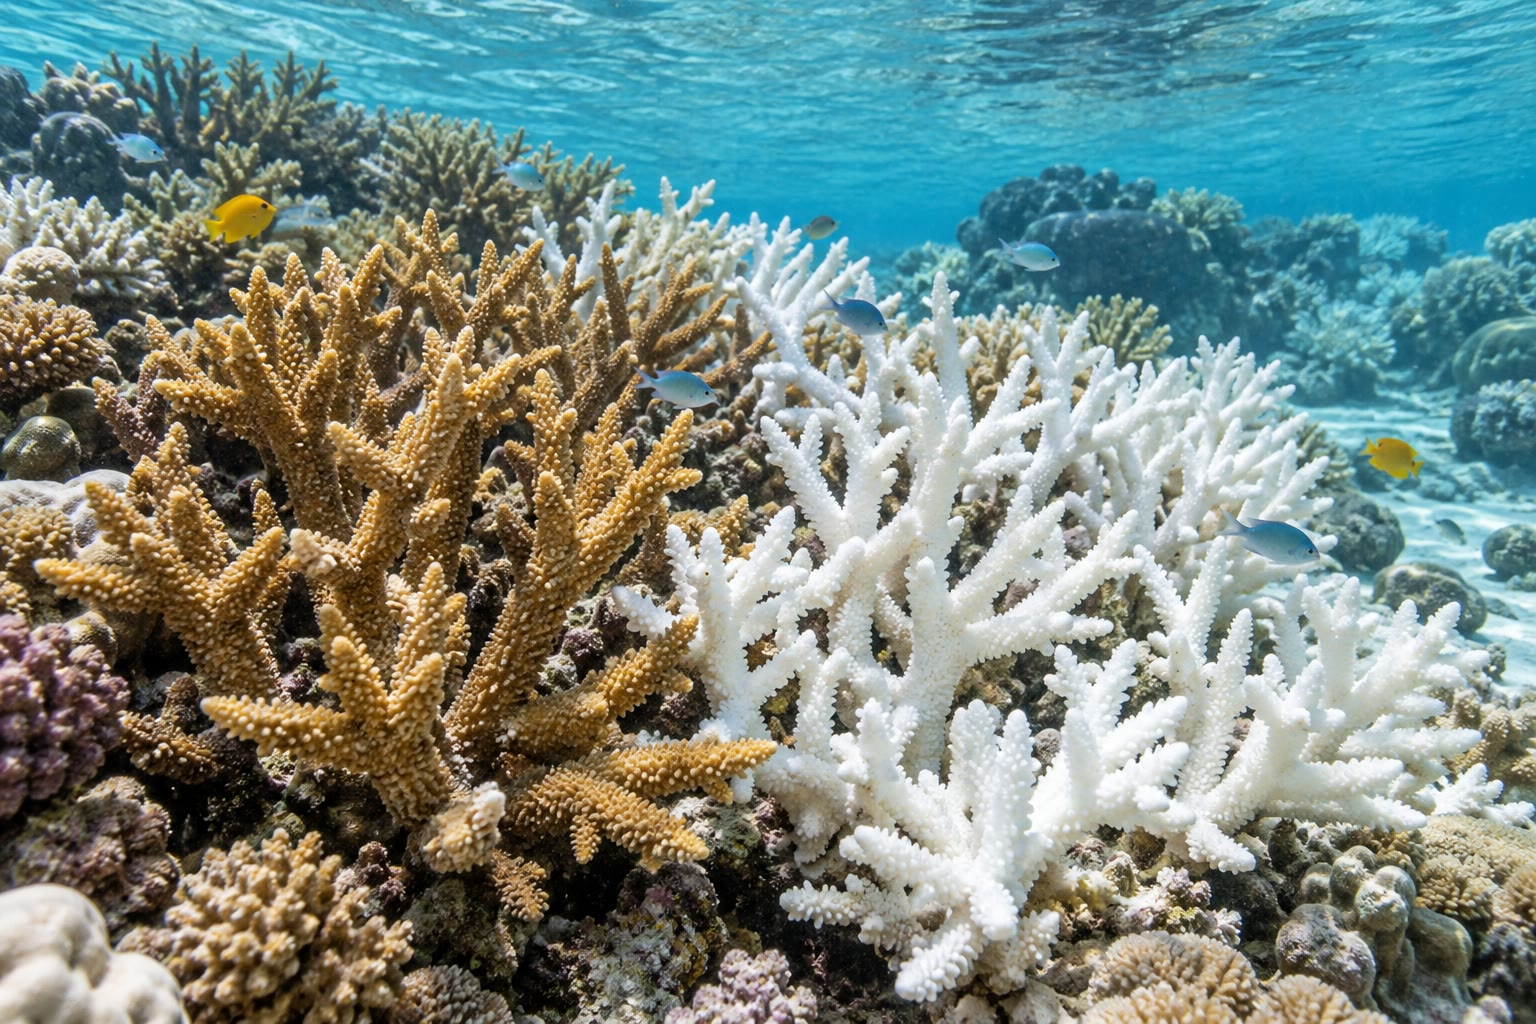
\includegraphics[width=0.44\linewidth]{images/book4/ai/b4-27-coral-bleaching.jpg}\hspace{0.04\linewidth}
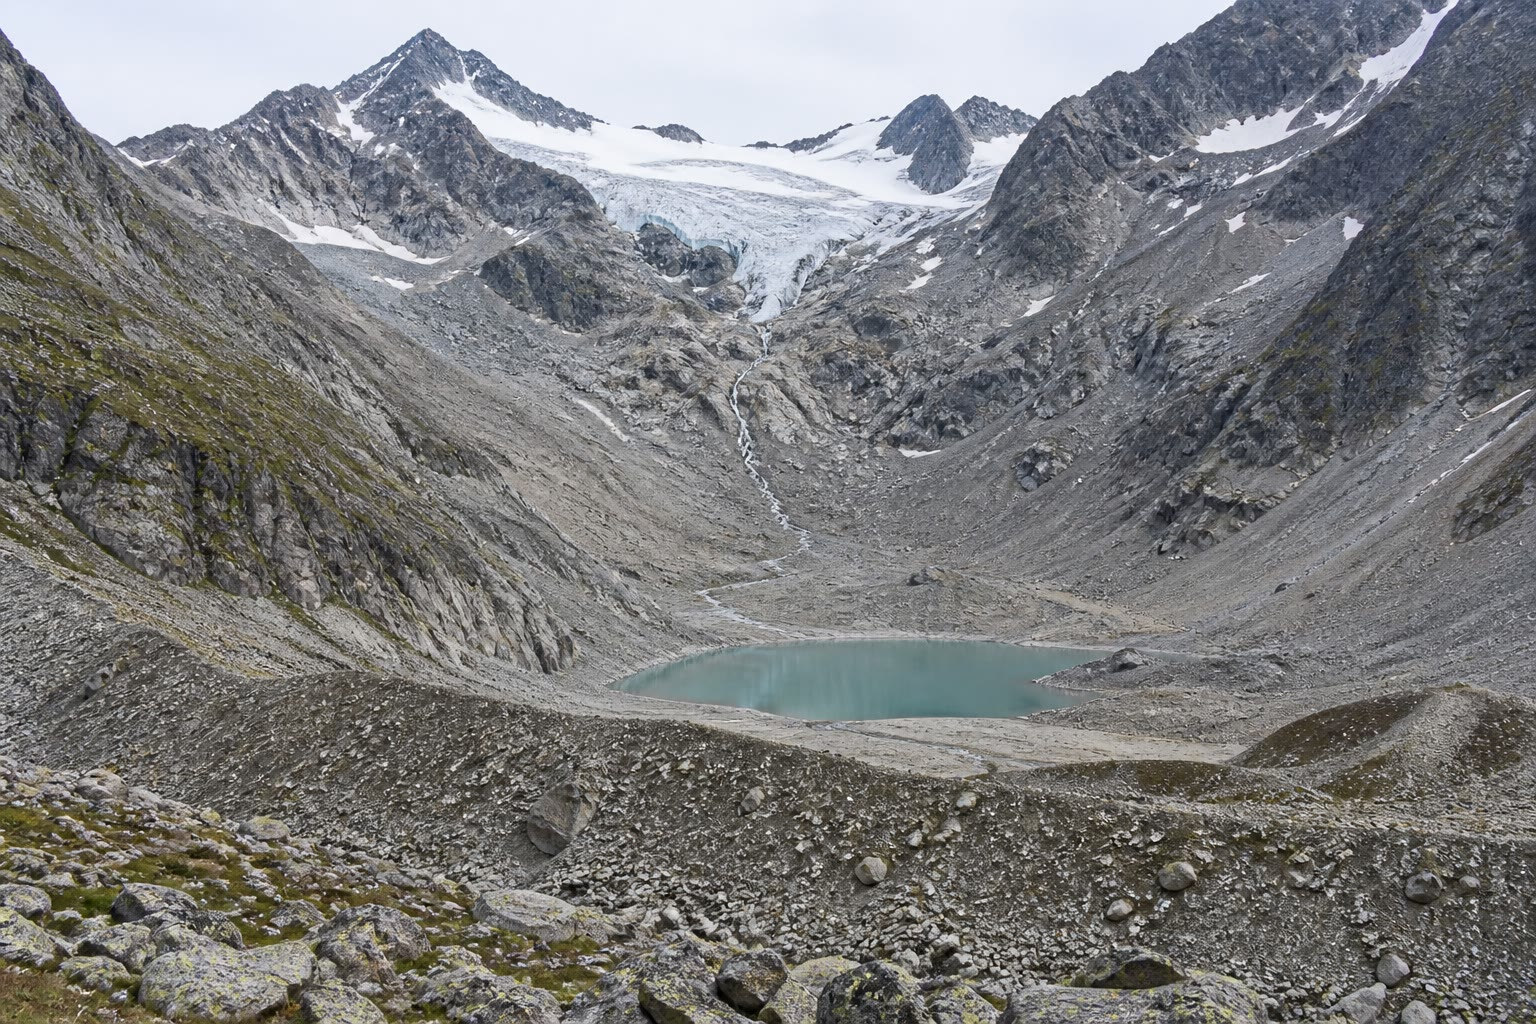
\includegraphics[width=0.44\linewidth]{images/book4/ai/b4-27-glacier-retreat.jpg}

{\small Dua termometer. Kiri: sebuah karang yang memutih, dengan rangka
putih karangnya tampak menembus jaringan yang telah kehilangan alganya.
Kanan: sebuah gletser lembah yang telah mundur naik lembahnya, lalu
meninggalkan batuan telanjang di tempat esnya berdiri seabad yang lalu.}
\end{omfigure}

\section{Rekeningnya: kepunahan dan taksirannya}

\begin{theorem}[Hubungan spesies--luas dan ongkos kehilangan habitat]\label{thm:b2:global-change:sar}
\index{hubungan spesies--luas}\index{laju kepunahan}%
\index{kehilangan habitat}\index{utang kepunahan}
Jumlah spesies yang ditemukan pada sebuah luas $A$ bertambah sebagai
sebuah pangkat luasnya, $S = cA^{z}$, dengan $z \approx 0.25$ bagi
pulau dan serpihan habitat (melipatduakan luasnya menambahkan seperlima
lebih banyak spesies; luas yang seratus kali lipat, tiga kali lebih
banyak). Jika sebuah habitat disusutkan menjadi sebagian sebesar $1 - h$ dari bentangannya, jumlah spesies yang akhirnya dapat ia tahan turun
menjadi $(1 - h)^{z}$ dari asalnya: kehilangan separuh habitatnya
berongkos \qty{16}{\%} spesiesnya, \qty{90}{\%} berongkos
\qty{44}{\%}, dan \qty{99}{\%} berongkos \qty{68}{\%}. Kehilangannya
tidak seketika --- yang bertahan hidup di dalam serpihannya bertahan
untuk sementara, yaitu sebuah \emph{\omterm{thm:b2:global-change:sar}{utang kepunahan}} yang dibayar
sepanjang berpuluh tahun ketika populasi yang kecil menyerah kepada
hanyutan dan \omterm{prop:b2:population-genetics:inbreeding}{silang dalam} pada \cref{ch:b2:population-genetics} --- dan
ia adalah dasar taksiran bahwa \omterm{thm:b2:global-change:sar}{laju kepunahan} sekarang adalah seratus
sampai seribu kali laju latar catatan fosilnya: yaitu kira-kira satu
spesies dari sejuta tiap tahun, berbanding beberapa ribu tiap tahun,
dari sekitar sepuluh juta, yang kini sedang hilang.
\end{theorem}
\begin{proof}
$S'/S = (A'/A)^{z} = (1 - h)^{z}$; dengan $z = 0.25$, $0.5^{0.25} =
0.84$, $0.1^{0.25} = 0.56$, $0.01^{0.25} = 0.32$. Hubungannya sendiri
bersifat empiris; eksponennya mencerminkan perimbangan, di pulaunya,
antara imigrasi spesies baru (yang turun ketika pulaunya terisi) dan
kepunahan spesies yang bermukim (yang naik ketika populasinya menyusut
bersama luasnya), yaitu kesetimbangan teori MacArthur dan Wilson.
\end{proof}
\begin{proof}[Bukti eksperimental]
Pulau kelompok Krakatau, yang disterilkan letusan tahun 1883, dijajah
kembali tumbuhan, burung, dan serangga dalam sebuah suksesi yang
mencapai, dalam lima puluh tahun, jumlah spesies yang diramalkan dari
luasnya; pulau kecil bakau yang diasapi Simberloff dan Wilson di
Florida pada tahun 1966 kembali kepada cacah spesies asalnya, dengan
spesies yang berbeda, dalam setahun. Hutan Atlantik Brasil, yang
disusutkan menjadi \qty{10}{\%} bentangannya, telah kehilangan atau
nyaris kehilangan bagian spesies burungnya yang diramalkan
hubungannya; dan pada tiap kelompok yang dinilai Lembaga Pelestarian
Dunia, seperempat sampai sepertiga spesiesnya terancam --- burung
\qty{13}{\%}, mamalia \qty{27}{\%}, amfibia \qty{41}{\%}, karang
\qty{44}{\%} --- dengan \omterm{thm:b2:global-change:sar}{kehilangan habitat} sebagai penyebab pertamanya,
serta perburuan, \omterm{prop:b2:global-change:invasion}{spesies invasif}, pencemaran, dan, kian meningkat,
iklimnya sebagai penyebab lainnya.
\end{proof}

\begin{omfigure}
\begin{tikzpicture}
\begin{loglogaxis}[
  width=0.68\linewidth, height=5.4cm,
  axis x line=bottom, axis y line=left,
  xmin=1, xmax=100000, ymin=5, ymax=200,
  xlabel={luas pulau (\unit{km^2})}, ylabel={spesies burung darat},
  xlabel style={font=\small, at={(axis description cs:0.5,-0.13)}, anchor=north},
  ylabel style={font=\small},
  tick label style={font=\small},
  clip=false,
]
\addplot[only marks, mark=*, mark size=2pt, omDef] coordinates {(1.5,9) (8,14) (35,22) (150,32) (400,37) (1200,52) (4000,70) (13000,92) (35000,125) (85000,160)};
\addplot[very thick, omThm, domain=1:100000, samples=2] {9*x^0.25};
\node[font=\scriptsize, omThm, anchor=north west, align=left] at (axis cs:2,120) {$S = 9A^{0.25}$: luas yang seratus\\ kali lipat, tiga kali\\ lebih banyak spesies};
\end{loglogaxis}
\end{tikzpicture}

{\small \omterm{thm:b2:global-change:sar}{Hubungan spesies--luasnya}, di sini bagi burung darat di pulau
sebuah kepulauan: sebuah garis lurus berkemiringan $z = 0.25$ pada
sumbu logaritmik. Pangkaslah sebuah habitat menjadi sepersepuluh dan ia
akan, pada waktunya, menyimpan sedikit lebih daripada separuh
spesiesnya.}
\end{omfigure}

\begin{proposition}[Penyerbuan, jasa, dan apa yang dapat dikerjakan]\label{prop:b2:global-change:invasion}
\index{spesies invasif}\index{jasa ekosistem}\index{mitigasi}\index{nol bersih}
Kapal, pesawat, dan perdagangan telah memindahkan ribuan spesies
melewati penghalang yang menjaganya tetap terpisah; kebanyakan gagal
mapan, tetapi segelintir yang berhasil --- kelinci di Australia,
kerang zebra di Danau Besar, ular pohon cokelat yang mengosongkan Guam
dari burungnya, jamur kitrid yang telah menggiring sembilan puluh
spesies amfibia menuju kepunahan --- menyebar sebagai sebuah muka yang
maju pada kecepatan tetap, $c =
2\sqrt{rD}$ bagi sebuah populasi yang
tumbuh pada laju $r$ dan memencar dengan koefisien difusi $D$ (tikus
air Skellam, yang dilepaskan di dekat Praha pada tahun 1905, meluas di
seluruh Eropa pada \qty{11}{km} tiap tahun, dengan jari-jari sebarannya
sebuah garis lurus terhadap waktunya). Melawan semuanya ini berdirilah
apa yang dikerjakan biosfernya bagi satu spesiesnya yang merepotkan:
\omterm{def:b2:angiosperm-reproduction:pollination}{penyerbukan} tiga perempat tanamannya, pemurnian air, pengendalian
banjir, pemfiksasian nitrogen dan pembuatan \omterm{def:b2:living-soil:soil}{tanah}, perikanan, karbon
yang ditahan di dalam hutan dan \omterm{def:b2:living-soil:soil}{tanahnya} --- yaitu \emph{\omterm{prop:b2:global-change:invasion}{jasa
ekosistem}} yang dinilai, di tempat sebuah harga dapat ditaruh padanya,
lebih besar daripada produk ekonomi dunianya. Apa yang dapat dikerjakan
mengikuti angkanya. Pemanasannya berhenti ketika pancaran bersihnya
berhenti, dan tidak sebelumnya: \omterm{thm:b2:biogeochemical-cycles:box}{model kotak} pada
\cref{ch:b2:biogeochemical-cycles} tidak membolehkan pembacaan lain
tentang \emph{\omterm{prop:b2:global-change:invasion}{nol bersih}}. Daratannya dapat menolong dalam batasnya ---
segigaton karbon tiap tahun dari penghutanan kembali dan \omterm{def:b2:living-soil:soil}{tanahnya}
selama beberapa dasawarsa, berbanding sepuluh dari bahan bakar
fosilnya --- dan spesiesnya dapat ditolong untuk berpindah, atau
disimpan di dalam cagar yang cukup besar dan terhubung sehingga
\omterm{thm:b2:global-change:sar}{hubungan spesies--luasnya} dan hanyutan populasi yang kecil tidak
menghabisinya. Perkakasnya adalah perkakas buku ini: \omterm{def:b2:population-genetics:frequencies}{genetika populasi}
cagarnya, persaingan penyerbunya, fenologi tanamannya, dan anggaran
\omterm{def:b2:living-soil:soil}{tanahnya}.
\end{proposition}

\begin{example}[Tiga masa depan]\label{ex:b2:global-change:scenarios}
Pancaran yang ditahan pada \qty{10}{GtC} tiap tahun sampai tahun 2100
menambahkan \qty{800}{GtC} kepada \qty{700}{} yang sudah dipancarkan:
$1.65\times 1.5 =
\qty{2.5}{\celsius}$ pada akhir abadnya dan masih
naik. Pancaran yang turun menjadi nol pada tahun 2070 menambahkan
kira-kira \qty{250}{GtC}: \qty{1.6}{\celsius}, lalu mendatar.
Melipatduakan pancarannya lebih dahulu, sebagaimana dikerjakan
dasawarsa awal abadnya, memberikan \qty{4}{\celsius} atau lebih.
Sebaran zona sedangnya berpindah \qty{200}{km} melampaui hari ini pada
keadaan yang pertama dan \qty{60}{km} pada yang kedua; musim
seminya datang dua puluh lima hari lebih awal, atau enam hari; pH
permukaannya mencapai $7.8$, atau tetap dekat $8.0$; dan taksiran
kepunahannya, yang bergantung pada habitat dan pemanasannya
bersama-sama, berjangkauan dari sepersepuluh sampai sepertiga
spesiesnya. Selisih antara masa depannya adalah luas kumulatif di bawah
satu kurva, yaitu jumlah keputusan yang belum dibuat.
\end{example}

\section{Latihan}

\begin{exercise}[$\star$]\label{exo:b2:global-change:1}
Nyatakan hubungan antara pemanasan dan \omterm{prop:b2:global-change:tcre}{pancaran kumulatifnya}, lalu
hitunglah pemanasannya bagi \omterm{prop:b2:global-change:tcre}{pancaran kumulatif} 700, 1000, dan
\qty{2000}{GtC}.
\end{exercise}

\begin{exercise}[$\star$]\label{exo:b2:global-change:2}
Definisikan derajat-hari dan \omterm{thm:b2:global-change:phenology}{ketakserasian fenologi}, dengan burung
sikatannya sebagai sebuah contoh.
\end{exercise}

\begin{exercise}[$\star$]\label{exo:b2:global-change:3}
Seberapa jauh isoterm berpindah ke atas bukit dan ke arah kutub tiap
derajat pemanasannya, dan mengapa sebuah spesies puncak gunung tidak
dapat mengikutinya?
\end{exercise}

\begin{exercise}[$\star$]\label{exo:b2:global-change:4}
Jelaskan dalam tiga kalimat mengapa menambahkan \ensuremath{\mathrm{CO_2}} ke lautnya
menurunkan pH dan karbonatnya, dan jasad mana yang dirugikan.
\end{exercise}

\begin{exercise}[$\star\star$]\label{exo:b2:global-change:5}
Hitunglah \omterm{prop:b2:global-change:tcre}{anggaran karbon} yang tersisa bagi \qty{1.5}{\celsius} dan
bagi \qty{2}{\celsius} dengan $\lambda = \qty{1.65}{\celsius}$ tiap
\qty{1000}{GtC} dan \qty{700}{GtC} yang sudah dipancarkan; ubahlah
keduanya menjadi tahun pada \qty{10}{GtC/yr}.
\end{exercise}

\begin{exercise}[$\star\star$]\label{exo:b2:global-change:6}
Musim semi menghangat pada $b = \qty{0.12}{\celsius}$ tiap hari dari
sebuah dasar \qty{5}{\celsius}; seekor ngengat memerlukan $K = 150$
derajat-hari. Hitunglah hari dari pelintasan dasarnya sampai
kemunculannya, dan majunya bagi sebuah pemanasan \qty{1.5}{\celsius}.
\end{exercise}

\begin{exercise}[$\star\star$]\label{exo:b2:global-change:7}
Sebaran sebuah tumbuhan membentang \qtyrange{800}{1400}{m} pada sebuah
gunung setinggi \qty{1800}{m} yang luasnya menyetengah tiap
\qty{300}{m} ketinggian. Setelah pemanasan \qty{3}{\celsius}, di
manakah pitanya dan berapa banyak luas yang telah ia hilangkan? Setelah
\qty{5}{\celsius}?
\end{exercise}

\begin{exercise}[$\star\star$]\label{exo:b2:global-change:8}
Hitunglah pH permukaannya dan kenaikan kepekatan ion hidrogennya pada
560, 800, dan \qty{1000}{ppm}, dari $\mathrm{pH} = 8.2 -
0.9\log_{10}(p/280)$.
\end{exercise}

\begin{exercise}[$\star\star$]\label{exo:b2:global-change:9}
Dengan $z = 0.25$, bagian spesies berapa yang akhirnya hilang ketika
\qty{70}{\%}, \qty{95}{\%}, dan \qty{99.9}{\%} sebuah habitat
dimusnahkan? Mengapa kehilangan seketikanya lebih kecil?
\end{exercise}

\begin{exercise}[$\star\star\star$]\label{exo:b2:global-change:10}
Seorang penyerbu tumbuh pada $r = 0.7$ tiap tahun dan memencar dengan
$D =
\qty{20}{km^2/yr}$. Hitunglah kecepatan mukanya dan waktu untuk
melintasi sebuah negeri selebar \qty{1000}{km}. Apa yang menyetengahkan
kecepatannya: menyetengahkan $r$ atau menyetengahkan $D$?
\end{exercise}

\begin{exercise}[$\star\star\star$]\label{exo:b2:global-change:11}
\omterm{thm:b2:global-change:sar}{Laju kepunahan} latarnya adalah 1 tiap sejuta spesies-tahun dan ada 8
juta spesies. Hitunglah kepunahan harapannya tiap tahun dan tiap abad
pada laju latarnya, dan pada 1000 kali laju latarnya. Bandingkan dengan
sepuluh ribu kepunahan yang terdokumentasi pada abad terakhir lalu
berilah ulasan tentang ketaksesuaiannya.
\end{exercise}

\begin{exercise}[$\star\star\star$]\label{exo:b2:global-change:12}
``Pemanasan berhenti ketika pancaran bersih berhenti.'' Benarkanlah
dari \omterm{thm:b2:biogeochemical-cycles:box}{model kotak} atmosfernya dan kesebandingan pemanasannya terhadap
\omterm{prop:b2:global-change:tcre}{pancaran kumulatifnya}, lalu katakan apa yang hilang dari hujahnya.
\end{exercise}

\section{Soal: Biosfer pada Tahun 2100}

\begin{problem}[{Soal akhir pekan --- dua jalur pancaran dibawa sampai
tahun 2100: pemanasan masing-masingnya, musim semi yang ia buat, jarak
yang ditempuh isotermnya, asam yang ia taruh di lautnya, dan spesies
yang ia bebankan kepada sebuah hutan, berakhir pada kedua pemanasannya,
kedua nilai pH-nya, dan bagian spesies yang hilang}]
\label{pb:b2:global-change:1}
Datanya. $\lambda = \qty{1.65}{\celsius}$ tiap \qty{1000}{GtC};
\qty{700}{GtC} dipancarkan sampai tahun 2020 (dengan pemanasan
\qty{1.2}{\celsius}). Jalur A: \qty{10}{GtC/yr} tetap sampai tahun
2100. Jalur B: turun secara lurus menjadi nol pada tahun 2070. Musim
semi menghangat pada $b = \qty{0.1}{\celsius}$ tiap hari di atas sebuah
dasar \qty{5}{\celsius}; sebatang pohon memerlukan $K = 200$
derajat-hari untuk berdaun, dan seekor burung ruaya tiba pada sebuah
tanggal tetap, 20 hari setelah pendaunan pohonnya pada tahun 2020. \omterm{prop:b2:global-change:range}{Laju
susut suhunya} \qty{6.5}{\celsius/km}; landaian lintangnya
\qty{0.65}{\celsius} tiap \qty{100}{km}. Lautnya: $\mathrm{pH} = 8.2 - 0.9\log_{10}(p/280)$;
\ensuremath{\mathrm{CO_2}} pada tahun 2100: \qty{600}{ppm} pada jalur A, \qty{420}{ppm} pada jalur B.
Sebuah daerah hutan seluas \qty{e5}{km^2} berisi 400 spesies pohon, $z = 0.25$,
kehilangan \qty{60}{\%} luasnya karena pembukaan lahan pada tahun 2100 pada jalur A dan
\qty{20}{\%} pada jalur B.

\medskip
\noindent\textbf{Bagian I --- Pemanasannya.}
\begin{enumerate}
  \item Hitunglah \omterm{prop:b2:global-change:tcre}{pancaran kumulatifnya} pada tahun 2100 pada tiap
        jalurnya.
  \item Hitunglah pemanasannya pada tahun 2100 pada tiap jalurnya.
  \item Hitunglah pemanasannya pada tahun 2050 pada masing-masingnya.
  \item Berapakah laju pemanasannya tiap dasawarsa pada jalur A?
        Bandingkan dengan \qty{0.2}{\celsius} tiap dasawarsa yang
        teramati.
  \item Pada jalur B, apakah pemanasannya berhenti pada tahun 2070?
        Mengapa, menurut kesebandingannya?
  \item \omterm{prop:b2:global-change:tcre}{Pancaran kumulatif} berapa yang bersesuaian dengan
        \qty{2}{\celsius}, dan pada tahun berapa jalur A melewatinya?
\end{enumerate}

\medskip
\noindent\textbf{Bagian II --- Musim seminya.}
\begin{enumerate}[resume]
  \item Hitunglah hari dari pelintasan dasarnya sampai pendaunannya
        pada tahun 2020.
  \item Hitunglah majunya pendaunannya, terhadap tahun 2020, pada
        tahun 2100 pada tiap jalurnya (dengan pemanasan terhadap tahun
        2020).
  \item Tanggal kedatangan burungnya tidak berubah. Hitunglah celah
        antara pendaunan dan kedatangannya pada tiap jalurnya pada
        tahun 2100.
  \item Ulat yang dibutuhkan burungnya memuncak 15 hari setelah
        pendaunannya lalu bertahan 10 hari. Pada jalur yang manakah
        burungnya masih menemukannya?
  \item Andaikan sebagai gantinya burungnya maju sebesar \qty{3}{d}
        tiap derajat. Hitung ulang celahnya pada jalur A.
  \item Nyatakan dalam satu kalimat mengapa ketakserasiannya, dan
        bukan pemanasannya sendiri, yang mengancam burungnya.
\end{enumerate}

\medskip
\noindent\textbf{Bagian III --- Sebarannya.}
\begin{enumerate}[resume]
  \item Hitunglah perpindahan isotermnya menurut ketinggian dan
        lintangnya pada tiap jalurnya, terhadap tahun 2020.
  \item Sebuah spesies pohon memencar \qty{100}{m} tiap tahun.
        Dapatkah ia mengikuti isotermnya ke arah kutub pada jalur A?
        Pada jalur B?
  \item Sebuah spesies menempati \qtyrange{1500}{1800}{m} pada sebuah
        gunung setinggi \qty{2000}{m}. Pada jalur A, di manakah pitanya
        duduk pada tahun 2100, dan apa yang terjadi?
  \item Luas gunungnya menyetengah tiap \qty{300}{m}. Hitunglah faktor
        luas yang dihilangkan spesies itu pada jalur B.
  \item Seekor ikan laut mengikuti isotermnya pada \qty{30}{km} tiap
        dasawarsa. Apakah itu cukup pada jalur A?
  \item Jelaskan mengapa tepi bawah sebuah sebaran mundur bahkan di
        tempat spesiesnya dapat menahan panasnya.
\end{enumerate}

\medskip
\noindent\textbf{Bagian IV --- Laut dan hutannya.}
\begin{enumerate}[resume]
  \item Hitunglah pH permukaannya pada tahun 2100 pada tiap jalurnya,
        dan kenaikan kepekatan ion hidrogennya sejak tahun 1750.
  \item \omterm{thm:b2:global-change:acid}{Keadaan kejenuhan} $\Omega$ permukaan tropikanya adalah 4 pada
        tahun 1750 dan turun sebagai $[\ensuremath{\mathrm{H^{+}}}]^{-1}$. Hitunglah ia
        pada tahun 2100 pada tiap jalurnya lalu katakan apa artinya
        bagi karangnya.
  \item Hitunglah jumlah spesies pohon yang akhirnya dapat ditahan
        daerah hutannya pada tiap jalurnya, dan jumlah yang hilang.
  \item Pemanasannya menambahkan kehilangan: andaikan tiap derajat di
        atas tahun 2020 menyingkirkan \qty{5}{\%} lagi spesies yang
        bertahan. Hitung ulang spesies yang tersisa pada tiap jalurnya.
  \item Berikan bagian dari 400 spesiesnya yang hilang pada tiap
        jalurnya.
  \item Manakah dari kedua penyebabnya, pembukaan lahan atau
        pemanasannya, yang menguasai pada tiap jalurnya?
  \item Nyatakan hasilnya: pemanasannya, pH-nya, dan bagian spesies
        pohon yang hilang pada tahun 2100 pada tiap jalurnya.
\end{enumerate}
\end{problem}
